\label{Chapter1}

\chapter{Introduction}

\section{Motivation}
A space exploration vehicle designed to move across the surface of a planet,
besides Earth, is called a planetary rover as of its ability to "rove over"
an unknown terrain.
Planetary rovers are used to collect valuable data and samples such as
images, dust and rocks, which are later analyzed by scientists to enrich
our understanding regarding the universe.

Past missions have sent robots to the Moon and Mars (Figure
\ref{fig:mars_sites}) with the NASA's Curiosity being the last rover to
land on Mars in 2012.
Future missions do not differ much, as new lunar rovers are about to launch
in the next years and Mars rovers are currently under development scheduled
to be sent to Mars in 2020.

Such missions utilize a great amount of time and effort to build,
launch and finally operate.
Our interest lies in the operational challenges caused by the fact
that no persistent communication to the base station can be achieved.
As an example, commanding messages can take up to 21 minutes to travel
between the Earth and Mars and restricted bandwidth can limit the number
of transmitted messages.
This compounded to the unpredictable and unsafe conditions of
a harsh terrain such as the Mars surface,
could lead to fatal system crashes of a costly mission.

Thus, we emphasize the need of a real time platform that will provide the
capability of autonomous operation with low supervision from ground control
as far as navigation is concerned.

\begin{figure}[h!]
    \centering
    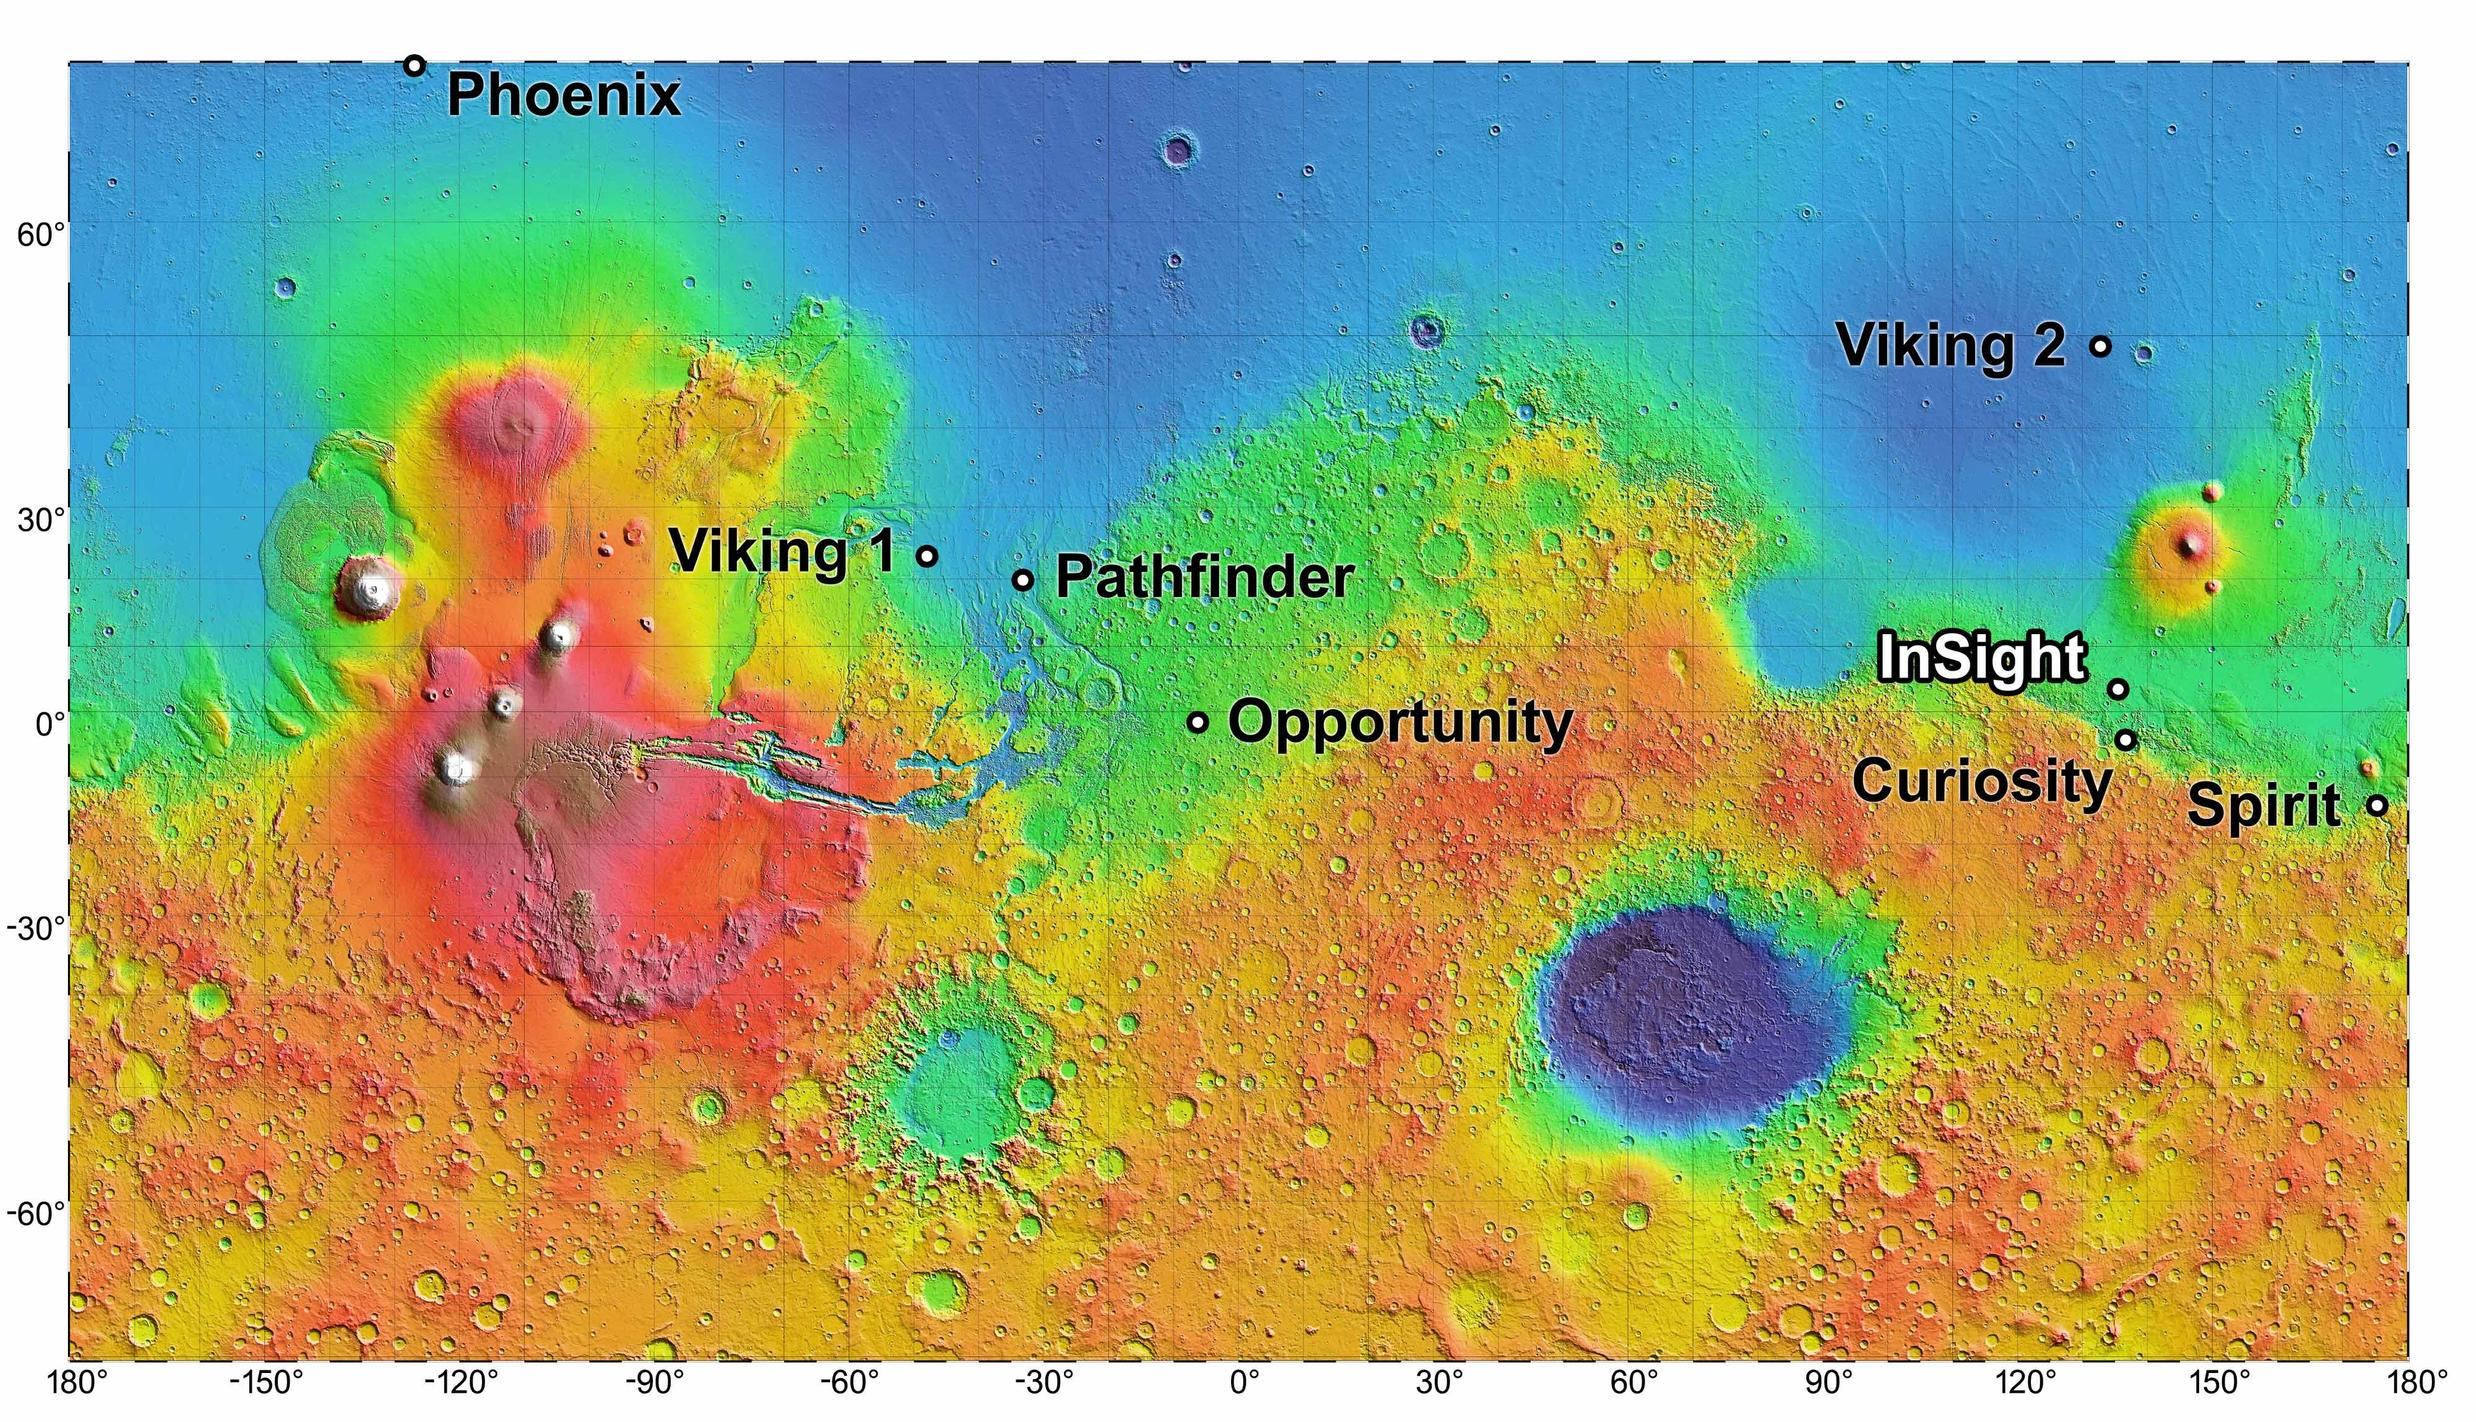
\includegraphics[scale=0.15]{mars_sites}
    \caption[Mars landing sites]{
        Mars landing sites of rovers and landers from NASA's past missions.
    }
    \label{fig:mars_sites}
\end{figure}

\section{Problem Statement}

In order to navigate autonomously in extreme terrains, rovers need to
accurately perceive the 3D environment around them based on sensory
information.
Terrains that classify as extreme are areas with high variance in elevation
and great morphological anomalies, including rocks and craters.

This thesis actively researches the challenges of perception in such terrains
in a planetary context and mainly focuses on two problems.
The first is the relative localization of the robot and the local mapping
of its surroundings in order to provide autonomous navigation capabilities
to it.
The second problem is the global localization of the robot, which is the
elimination of the accumulated drift from relative localization in long
range scenarios.

Specifically, given as inputs:
\begin{enumerate*}[label=(\roman*)]
    \item an initial prediction about the robot's movement,
    \item a detailed 3D representation of the close surroundings of the robot
        and
    \item an a priori low resolution map of the greater area,
\end{enumerate*}
the purpose is to produce:
\begin{enumerate*}[label=(\roman*)]
    \item an accurate estimation of the position and orientation of the
        robot in a global reference frame and
    \item a local (robot-centric) map that represents the height of
        the environment.
\end{enumerate*}

\subsection{Presumptions}

In order to tackle the aspect of the problem that is of most interest,
we first assume the following:

\begin{itemize}
    \item a low resolution global map is available to the system at any time
    \item the initial global position of the robot is known
    \item the environment is static, i.e. is does not contain any
        moving objects
    \item the environment is unknown, i.e. there are no high resolution
        a priori maps available
    \item the terrain is single layered, i.e. there are no bridges or caves
\end{itemize}

\section{Literature Review}

\subsection{Simultaneous Localization and Mapping}

In early robotics research, localization and mapping were tackled
independently.
This is related to the fact that they have a cyclic inter-dependency.
On the one hand, a map can only be created when the robot’s pose is known,
whilst on the other hand, we need an accurate map representation in order to
perform localization.
Nevertheless, both tasks usually need to be performed simultaneously:
in this case we speak of Simultaneous Localization and Mapping (SLAM).

SLAM problems can be distinguished in several ways \parencite{Jefferies2008}:
\begin{itemize}
    \item \textbf{Volumetric versus feature-based}:
        Volumetric SLAM allows a realistic reconstruction of the environment,
        since the map is high-dimensional and sampled at a high resolution.
        In feature-based SLAM, the map is comprised of sparse features
        that are extracted from the sensors.
        Although featured-based techniques tend to be more efficient,
        they are not commonly used in autonomous navigation tasks.
    \item \textbf{Static versus dynamic}:
        Static SLAM algorithms make the assumption that the environment
        does not change during separate observations in time.
        In contrast, dynamic SLAM approaches assume an environment that
        can contain moving objects and usually treat them as
        measurement outliers.
    \item \textbf{Active versus passive}:
        In passive SLAM algorithms, the SLAM algorithm cannot affect the
        movement of the robot which is purely observing.
        In active SLAM, the robot actively explores its environment in
        the pursuit of an accurate map.
        Active SLAM methods tend to yield more accurate maps in less time,
        but they constrain the robot motion.
        There exist also hybrid techniques in which the SLAM algorithm
        controls only the pointing direction of the robot's sensors,
        but not the motion direction.
    \item \textbf{Full vs online}:
        Full-SLAM approaches calculate the entire path and construct the
        map as soon as the data acquisition is completed.
        Online-SLAM, on the other hand, assumes that the previous poses are a
        continuous estimate and a map is built on the fly.
\end{itemize}

As such, an autonomous planetary rover would require an online and volumetric
SLAM method to fulfill its navigation tasks and could also safely assume a
static environment.
Depending on its exploration capabilities, an active or passive method
could be selected.

In order to solve the SLAM problem, many approximate solution methods
have been developed.
These include probabilistic approaches, such as particle filters or extended
Kalman filters (EKF), optimization approaches, such as graph-based solutions,
as well as scan matching techniques.

Particle filters or Sequential Monte Carlo (SMC) filters
\parencite{Doucet2001, Murphy1999}, are a set of genetic type statistical
approaches to solving the filtering problem.
The particle filter is a tool for tracking the state of a dynamic system,
even when the state is not fully observable.
Particle filters is in practice a Bayes filter that uses a prediction
and update cycle to estimate the state of a dynamical system from
sensor measurements, and has similar applications as the Kalman filter,
but handles large dimensionality better \parencite{Thrun2005}.

Interestingly, this approach can be used to solve both the online and
full-SLAM problem simultaneously using a grid-map based approach.
Particle filters have become one of the most common approaches of
solving the SLAM problem in modern robotics.
Popular algorithms include FastSLAM \parencite{Montemerlo2002} which
uses a class of particle filters called Rao-Blackwellized particle filters
(RBPFs) \parencite{Doucet2000, Murphy2001} and GMapping
\parencite{Grisettiyz2005} which uses a combination of particle filters
and scan matching.

Scan matching is one of the oldest and easiest to implement methods used
to solve the SLAM problem using Occupancy Grid Maps (OGM) - maps that
represent the continuous space using a discrete uniform grid.
In scan matching, the position of the robot is calculated by matching,
i.e. computing the transformation, between the current and previous
sensor scans.
Based on this concept, numerous implementations and variations have
been developed due to its simplicity \parencite{Rusinkiewicz2001, Brenna2008}.

Another popular approach for feature based maps is the Extended Kalman Filter,
which applies the EKF to online-SLAM using maximum likelihood data association.
The EKF assumes the noise to be Gaussian for motion and perception.
EKF integrates out the robot's pose as the robot moves, and therefore only
keeps track of the current pose \parencite{Thrun2005}.

Finally, the full-SLAM problem can be solved using graph based approaches
such as Graph-SLAM.
In Graph-SLAM the robot poses are represented as a graph where the
nodes correspond to the poses of the robot at different points in time,
and the edges represent constraints between the poses \parencite{Thrun2005}.
The latter are obtained from observations of the environment or from
movement actions carried out by the robot.
The whole problems boil down to solving a large optimization problem.
The graph can be shown to be a sparse graph of nonlinear constraints.
Graph-SLAM needs to keep track of all poses and measurements at all times,
but since it is an offline approach, it does not need to perform computations
while collecting data.

\subsection{Planetary Absolute Localization}

Precise localization in a planetary terrain without any communication
assistance from the Earth is considered an essential feature in
long-range scenarios (e.g. 10 km and up).
A series of matching techniques have been examined in order to align the
global and local maps.

\subsubsection{Skyline-based}

Skyline based methods attempt to estimate the global position of a rover
by matching the skyline of the horizon, with skylines extracted from
the global map \parencite{Stein1992, Cozman1997}.
The VIPER algorithm \parencite{Cozman2000} is a global localization
algorithm that matches the horizon skyline signature captured by a
panoramic picture acquired by the rover, to predicted skylines signatures
at various positions on the global map.
It has been proven efficient in the global localization problem,
where the rover's initial position is not known, and is rather quick because
it precomputes the skylines of the global map in an offline fashion.
It yields an estimation accuracy of $\SI{100}{\m}$ to $\SI{150}{\m}$ on a
$\SI{30}{\m \per pixel}$ digital elevation map (DEM).
However, this approach is not behaving smoothly in cases where the horizon
is hardly detectable and when the DEM has not covered an area large enough
to allow the prediction of the skyline.

\subsubsection{Feature-based}

Featured-based approaches, in general, initially extract interest points
from the global and local maps and then they match them in search of
global-local feature correspondences.

MOGA \parencite{Carle2010} is another solution to the long-range localization
problem with an approach similar to VIPER's, but uses 3D maps
instead of 2D images.
In particular, it was observed that capturing 3D peak features has
better alignment performance.
The methodology was tested with real data, including 37 LiDAR scans of
terrain from a Mars-Moon analog site on Devon Island, Nunavut.
LiDARs though, are hardly used in planetary rovers due to the heavy
weight and high power consumption, as well as their big data range,
that results to heavy calculations.

Moreover, in order to autonomously localize a Mars rover,
an integrated Visual Odometry and Bundle Adjustment method \parencite{Li2007}
was proposed that automatically selects tie-points, such as rocks,
and links the ground images acquired at multiple rover sites into
an image network.
Test results using MER (Mars Exploration Rovers) data showed that the
proposed method achieved promising results for medium-range (up to
$\SI{26}{\m}$) traverse segments.
However, significant differences in resolution between orbital and
ground imagery has proven this approach unable to be fully automated.

With the aim to solve the resolution issues, a method using orbital and
ground images was proposed \parencite{Hwangbo2009}, in which
high-resolution orthographic photos and DEMs are generated as soon as the
orbital stereo images are acquired.
A ground image network is also constructed using inter-stereo matching.
From both types of imagery, a few landmarks are identified to be used as
ground control points for the integration of the orbital and ground
image networks.
Finally, distribution pattern matching is implemented for rocks detected
from orbital and ground imagery.
The rover position is adjusted based on a 2D affine transformation
obtained from rock pattern matching.
Experiments in MER data achieve a success rate of up to $50\%$, since
there are terrain restrictions: desert areas with no rocks,
or on the contrary very rough areas, in which rocks are hardly
defined are difficult to handle.

More examples of feature-based matching techniques are spin images
\parencite{Johnson1997} and point fingerprints \parencite{Sun2003}.
These methods create a descriptor for each extracted feature based on the
geometry.
A spin-image descriptor is a two dimensional histogram that
represents the distances of surrounding map points to the local tangent
plane and normal vector at the feature’s location.
When comparing two descriptors, a correspondence is made if they are
sufficiently similar.
Similar well-known descriptors are the SIFT \parencite{Lowe2004}
and SURF \parencite{Bay2006}, which can be used in order to analyze images.

\section{Thesis Objectives and Outline}

\subsection{Research Objectives}

The main objectives of this thesis in terms of research are:

\begin{itemize}
    \item to utilize SLAM techniques for the localization and mapping
        of a planetary rover
    \item to develop a novel technique for minimizing the localization
        drift with global map matching
    \item to determine under which circumstances (i.e. resolutions of
        local and global maps) can the orbital imagery be useful for
        solving the SLAM problem
    \item to examine and quantify the gains (i.e. high resolution map for
        navigation purposes and absolute localization) and loses
        (i.e. processing overhead) of such approach.
\end{itemize}

\subsection{Outline}

The remainder of this thesis is organized as follows:
\begin{itemize}
    \item \textbf{Chapter 2} introduces a detailed approach for solving the
        SLAM problem in a planetary context using global map matching,
    \item \textbf{Chapter 3} deals with the implementation details and
        the tools used to develop a working system overall,
    \item \textbf{Chapter 4} presents the results of the experiments that
        were carried out in order to validate the approach and
    \item \textbf{Chapter 5} concludes with a summary, thoughts about future
        directions as well as possible applications.
\end{itemize}

